\chapter{Introduction}


\section{Motivation and Background}

% Autonomous Vehicle

Modern technologies have the potential to create a paradigm shift in the vehicle-driver relationship with advanced automation changing the driver role from "driving" to "supervising". To design new driver environments that caters for these emerging technologies, traditional approaches identify current human and technical constraints to system efficiency and create solutions accordingly. However, there are two reasons why such approaches are limited within the technologically-evolving automotive domain. First, despite significant progress in the development of system theory and methods, the application of these methods is largely constrained to the existence of a current system. Second, there are few structured approaches for using the analysis results to support design. In this paper, an attempt is made to overcome these challenges by developing and implementing a method for analyzing and designing a highly autonomous commercial vehicle. 

An autonomous vehicle has great potential to improve driving safety, comfort and efficiency and can be widely applied in a variety of fields, such as road transportation, agriculture, planetary exploration, military purpose and so on \cite {WANG2015727}. The past three decades have witnessed the rapid development of autonomous vehicle technologies, which have attracted considerable interest and efforts from academia, industry, and governments. Particularly in the past decade, contributing to significant advances in sensing, computer technologies, and artificial intelligence, the autonomous vehicle has become an extraordinarily active research field. During this period, several well-known projects and competitions for autonomous vehicles have already exhibited autonomous vehicles' great potentials in the areas ranging from unstructured environments to the on-road driving environments \cite{AutonomousStructured} \cite{DrivingUrban2008}.

% Adaptive Cruise Control

In this paper, we are aiming for an autonomous driving system allowing the vehicle to smartly choose the driving behaviors, such as adjusting the speed and changing the lane. In fact, Adaptive cruise control (ACC), a radar-based system, has been designed to enhance driving comfort and convenience by relieving the need to continually adjust the speed to match that of a preceding vehicle. The system slows down when it approaches a vehicle with a lower speed, and the system increases the speed to the level of speed previously set when the vehicle upfront accelerates or disappears (e.g., by changing lanes). Traditional methods have proved the reliability in several cases though the use is still quite limited and only for expected scenarios. While, currently, artificial intelligence especially deep reinforcement learning is aggressively expanding the border of human's imagination and machine's autonomy. Thus, a new highway adaptive cruise control (HACC) is proposed for autonomous vehicles with the help of deep reinforcement learning.

\section{Literation Review}

% The rise of Deep Q Learning

Google's DeepMind published its famous paper Playing Atari with Deep Reinforcement Learning \cite {Mnih2015AtariNature}, in which they introduced a new algorithm called Deep Q Network (DQN for short) in 2013. It demonstrated how an AI agent can learn to play games by just observing the screen without any prior information about those games. The result turned out to be pretty impressive. This paper opened the era of what is called "deep reinforcement learning", a mix of deep learning and reinforcement learning.

% Reinforcement Learning
Reinforcement Learning is a type of machine learning that allows you to create AI agents that learn from the environment by interacting with it. Just like how we learn to ride a bicycle, this kind of AI learns by trial and error. As seen in Fig. \ref {fig:deepmind}, the brain represents the AI agent, which acts on the environment. After each action, the agent receives the feedback. The feedback consists of the reward and next state of the environment. The reward is usually defined by a human. If we use the analogy of the bicycle, we can define reward as the distance from the original starting point.

\begin{figure}[h] 
\centering
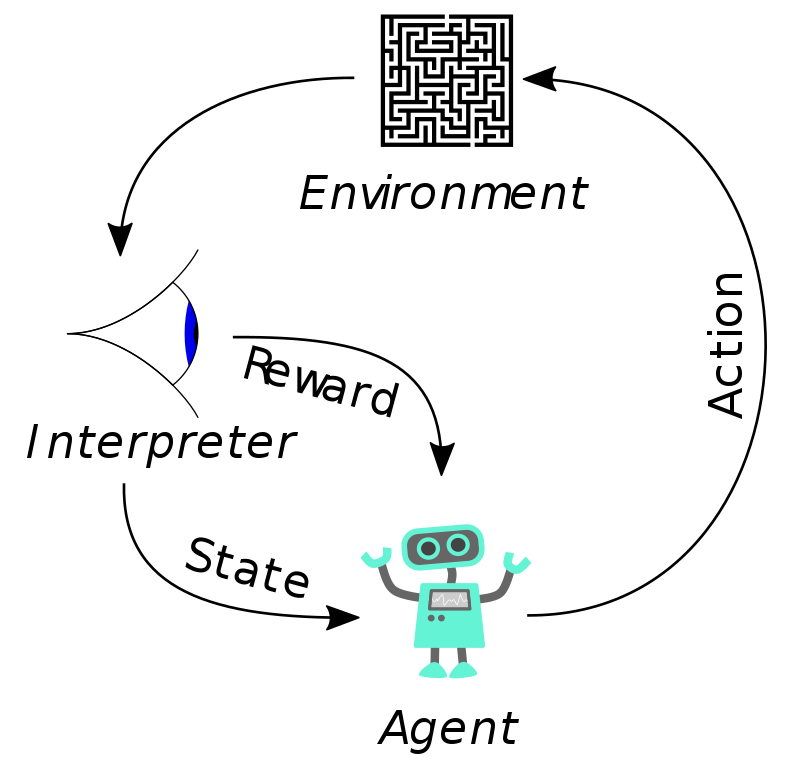
\includegraphics[width=0.5\textwidth]{figs/ch1/Reinforcement_learning_diagram}
\caption{How an agent interacts with the environment.}
\label{fig:deepmind}
\end{figure}

Standard model-based methods for robotic manipulation might involve estimating the physical properties of the environment, and then solving for the controls based on the known laws of physics \cite{OK-Robot-1987} \cite{Predictive2014} \cite{PlanningFramework2012}. This approach has been applied to a range of problems. Despite the extensive work in this area, tasks like pushing an unknown object to a desired position remain a challenging robotic task, largely due to the difficulties in estimating and modeling the physical world \cite{IROS2016}. Learning and optimization-based methods have been applied to various parts of the state-estimation problem, such as object recognition \cite{Visual1995}, pose registration \cite{ObjectRecognition2009}, and dynamics learning \cite{DynamicsDoor2013}.

However, estimating and simulating all of the details of the physical environment is exceedingly difficult, particularly for previously unseen objects, and is arguably unnecessary if the end goal is only to find the desired controls. For example, simple rules for adjusting motion, such as increasing force when an object is not moving fast enough, or the gaze heuristic \cite{FieldersNature2003}, can be used to robustly perform visuomotor control without an overcomplete representation of the physical world and complex simulation calculations. Our work represents an early step toward using learning to avoid the detailed and complex modeling associated with the fully model-based approach.

Several works have used deep neural networks to process images and represent policies for robotic control, initially for driving tasks \cite{AutonomousLand1989} \cite{LongrangeVision2009}, later for robotic soccer \cite{RobotSoccer2009}, and most recently for robotic grasping \cite{Grasp2016} \cite{RooticGrasping2016} and manipulation \cite{Visuomotor2016}. Although these model-free methods can learn highly specialized and proficient behaviors, they recover a task-specific policy rather than a flexible model that can be applied to a wide variety of different tasks. The high dimensionality of image observations presents a substantial challenge to model-based approaches, which have been most successful for low-dimensional non-visual tasks \cite{PolicySearch2011} such as helicopter control \cite{HeliNg2007}, locomotion \cite{Trajectory2012}, and robotic cutting \cite{Deepmpc2015}. Nevertheless, some works have considered modeling high-dimensional images for object interaction. For example, Boots et al. \cite{Predictive2014} learn a predictive model of RGB-D images of a robot arm moving in free space.

% CACC

A lot of related work has been done in recent years in the design of CACC systems. Regarding the vehicle-following controller, Hallouzi et al. [8] did some research as part of the CarTalk 2000 project. These authors worked on the design of a longitudinal CACC controller based on vehicle-to-vehicle communication. They showed that inter-vehicle communication can help reduce instability of a platoon of vehicles. In the same vein, Naranjo and his colleague [14] worked on designing a longitudinal controller based on fuzzy logic. Their approach is similar to what we did with reinforcement learning for our low-level controller. Forbes has presented a longitudinal reinforcement learning controller [5] and compared it to a hand-coded following controller. He showed that the hand-coded controller is more precise than its RL controller but less adaptable in some situations. However, Forbes did not test explicitly communication between vehicles to improve its longitudinal controller to a multi-vehicle environment (which will be the focus of our future work). Our approach will also integrate our low-level controllers with a high-level multiagent decision making algorithm, which was not part of Forbes' work.

Regarding the reinforcement learning in a vehicle coordination problem, Unsal, Kachroo and Bay \cite{CACC1999} have used multiple stochastic learning automata to control the longitudinal and lateral path of a vehicle. However, the authors did not extend their approach to the multi-agent problem. In his work, Pendrith \cite{DistributedRL-Traffic2000} presented a distributed variant of Q-Learning (DQL) applied to lane change advisory system, that is close to the problem described in this paper. His approach uses a local perspective representation state which represents the relative velocities of the vehicles around. Consequently, this representation state is closely related to our 1-partial state representation. Contrary to our algorithms, DQL does not take into account the actions of the vehicles around and updates Q-Values by an average backup value over all agents at each time step. The problem of this algorithm is the lack of learning stability.

On the other hand, our high level controller model is similar to Partially Observable Stochastic Games (POSG). This model formalizes theoretically the observations for each agent. The resolution of this kind of games has been studied by Emery-Montermerlo \cite{GameControl2005}. This resolution is an approximation using Bayesian games. However, this solution is still based on the model of the environment, unlike our approach which does not take into account this information explicitly since we assume that the environment is unknown. Concerning the space search reduction, Sparse Cooperative Q-Learning \cite{Sparse2004} allows agents to coordinate their actions only on predefined set of states. In the other states, agents learn without knowing the existence of the other agents. However, unlike in our approach, the states where the agents have to coordinate themselves are selected statically before the learning process. The joint actions set reduction has been studied by Fulda and Ventura who proposed the Dynamic Joint Action Perception (DJAP) algorithm \cite{JointAction2003}. DJAP allows a multi-agent Q-learning algorithm to select dynamically the useful joint actions for each agent during the learning. However, they concentrated only on joint actions and they tested only their approach on problems with few states.

Introducing communication into decision has been studied by Xuan, Lesser, and Zilberstein \cite{Multi-agentCooperation2001} who proposed a formal extension to Markov Decision Process with communication where each agent observes a part of the environment but all agents observe the entire state. Their approach proposes to alternate communication and action in the decentralized decision process. As the optimal policy computation is intractable, the authors proposed some heuristics to compute approximation solutions. The main differences with our approach is the implicit communication and the model-free learning. More generally, Pynadath and Tambe \cite{Communicative2002} have proposed an extension to distributed POMDP with communication called COM-MTDP, which take into account the cost of communication during the decision process. They presented complexity results for some classes of team problems. As Xuan, Lesser, and Zilberstein \cite{Multi-agentCooperation2001}, this approach is mainly theoretical and does not present model-free learning. The locality of interactions in a MDP has been theoretically developed by Dolgov and Durfee \cite{Makov2004}. They presented a graphical approach to represent the compact representation of a MDP. However, their approach has been developed to solve a MDP and not to solve directly a multi-agent reinforcement learning problem where the transition function is unknown.


\section{Thesis Outline}

The goal of this thesis is to provide operational specifications for the development of a level 4 capable AVRP. This section will present the chapters and subsections of this thesis and provide a brief summary of those sections.

Chapter 2 details the system specifications required to develop an AVRP, based off feedback from faculty and researchers at Virginia Tech.
\begin{itemize}
\item \textbf {Section 2.1 Interdisciplinary Design Needs:} Looks at the feedback given by faculty and researchers at Virginia Tech and what kinds of research they would like to utilize an AVRP for. Breaks down the research desires into the basic needs for an AVRP. Some of the feedback is broken down with more background information.
\end{itemize}

Chapter 3 dives into the hardware and sensing side of an AVRP and lays out a discussion of the technology needed, such as DBW, navigation, sensing, communication, computing, power bus, and external mounting racks. It then reviews additional design considerations that need to be taken into consideration when designing an AVRP. Chapter 3 is laid out as follows:
\begin{itemize}
\item \textbf {Section 3.1 Drive By Wire:} Discusses the DBW system and significant design parameters to be considered. Lays out the specifications of the by wire system on a base platform at Virginia Tech. Presents a high level overview of DBW system.
\item \textbf {Section 3.2 Navigation:} Discusses different combinations for navigation, such as GPS/ INS and GPS/IMU, and some of the characteristics associated with each, as well as navigation via dead reckoning. Correction techniques such as DGPS and DGPS with RTK are reviewed. Hardware mounting is briefly mentioned.
\item \textbf {Section 3.3.1 LIDAR:} Discusses how LIDAR works. 2D and 3D LIDAR is discussed. Discusses certain characteristics such as range, accuracy, field of view, number of re- turns, intensity, advantages and disadvantages. Reviews possible mounting locations.
\item \textbf {Section 3.3.2 Radar:} Discusses how radar works and its usefulness on an AVRP. Talks about the different operation frequencies used in autonomy and how they affect performance, as well as other advantages and disadvantages. Possible mounting locations are discussed.
\item \textbf {Section 3.3.3 Ultrasonic:} Discusses the use of ultrasonic sensors and their advantages and disadvantages. Reviews their range and mounting locations.
\item \textbf {Section 3.3.4 Cameras:} Discusses different camera types and capability they bring to an AVRP. Goes over camera specifications for consideration. Reviews potential mounting locations.
\item \textbf {Section 3.3.5 Wheel Speed and Steering Angle Sensors: }Discusses wheel encoders and steering angle sensors and how they complement other sensing and systems.
\item \textbf {Section 3.4.1 Communication:} Presents different communication buses for intra-vehicle communication. Provides an overview, specs, and explanation of an AVRP communication bus structure. Reviews the need for an emergency stop system.
\item \textbf {Section 3.4.2 Computers:} Addresses computing for the end users by presenting bench- marks and guide posts for consideration when determining computational needs for the end user of an AVRP.
\item \textbf {Section 3.5 Base Sensor Suite Design:} Specs out the base sensor suite for an AVRP and the capabilities it allows for the AVRP without user added sensors.
\item \textbf {Section 3.6 Power Bus:} Discusses AVRP power bus layout to provide power to all internally and externally mounted hardware and sensors. Provides an estimate of power need for base sensor suite and an example sensor suite.
\item \textbf {Section 3.7.1 Front Universal Mounting Racks:} Reviews details and modifications made for adding front universal mounting rack to AVRP.
\item \textbf {Section 3.7.2 Rear Universal Mounting Racks:} Reviews details and modifications made for adding rear universal mounting rack to AVRP.
\item \textbf {Section 3.7.3 Roof Universal Mounting Racks:} Reviews details and modifications made for adding roof top universal mounting rack to AVRP.
\item \textbf {Section 3.7.4 Mounting Rack Vibration:} Discusses vibration concerns and performs example natural frequency calculations for the front and rear universal mounting racks.
\item \textbf {Section 3.7.5 Interchanging Hardware:} Discusses design considerations for hardware and sensors to be added to the mounting racks, such as roof top penetrations, routing wires, adapter brackets, etc.
\item \textbf {Section 3.8 Additional Design Considerations:} Discusses other AVRP design considerations, such as funding, team structure, base vehicle variability, hardware selection properties, etc.
\end{itemize}

Chapter 4 reviews the base vehicle research capabilities and contains a testing plan ideas for an AVRP. Chapter 4 is a follows:

\begin{itemize}
\item \textbf {Section 4.1 Base Vehicle Research Capabilities:} Reiterates on the base platform capabilities without any user added sensors.
\item \textbf {Section 4.2 Testing Plan Overview:} Discusses testing plan options for an AVRP and how it can be validated for use for its researchers.
\end{itemize}

Chapter 5 contains the conclusion and areas for future work. Chapter 5 sections are as follows:

\begin{itemize}
\item \textbf {Section 5.1 Conclusion:} Reviews the design of an AVRP, hardware, sensors, and modifications to make it adaptable to a researcher?s needs.
\item \textbf {Section 5.2 Future Work:} Looks at areas relevant to an AVRP in which further research can be conducted.
\end{itemize}

%%%%%%%%%%%%%%%%%%%%%%%%%%%%%%%%%%%%%%%%%%%%%%%%%%%%%%%%%%%%%%%%%%%%%%%%%%%%%%%%%%%%%%%%%%%%%%%%%%%%



%\bibliographystyle{plainnat}
%\markright{\textit{Bibliography}}
%\renewcommand{\chaptername}{}
%x\bibliography{KL-Thesis}

\vfill

